\documentclass[10pt,a4paper]{article}
\usepackage[utf8]{inputenc}
\usepackage{amsmath}
\usepackage{amsfonts}
\usepackage{amssymb}
\usepackage{graphicx}
\usepackage{a4wide}
\usepackage{pgfplots}

\begin{document}
	\section*{Kriterien für die Lesbarkeitsanalyse}
	\subsection*{Wortlänge}
	Hierfür wird zunächst die durchschnittliche Wortlänge analysiert und normiert. Sei $ W $ die Menge aller Wörter $ w_i $ im zu analysierenden Text mit Wortlänge $wl_i= |w_i| $. Die minimale Wortlänge ist 1 (bzw. 2 im Deutschen), die maximale ist $ l_{max}=max(|w_i|) $ bzgl. aller Wörter $ w_i\in W $. Der Lesbarkeitswert jedes Wortes wird normiert durch $ \frac{|w_i|}{l_{max}}$ und z.B. auf Farbwerte zwischen blau $ (32,62,181) $, weiß und rot $ (186,57,44) $ abgetragen.\\

\pgfplotsset{compat=1.10}
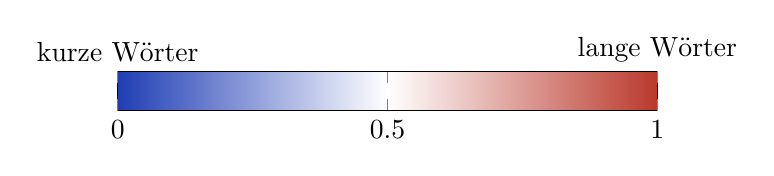
\begin{tikzpicture}
\begin{axis}[
colormap={lolmap}{[1cm] 
	rgb255(0cm)=(32,62,181) color(5cm)=(white) rgb255(10cm)=(186,57,44)}, colorbar horizontal, colorbar/width=.5cm, 
	colorbar style={xtick={0,.5,1},
	xlabel near ticks, 
	extra x ticks={0,1},
	extra x tick labels={kurze Wörter, lange Wörter}, 
	extra x tick style={ticklabel pos=right}   
	},
	hide axis
]
%\addplot[mesh, point meta=y, line width=4mm, samples=150] {x^2}; % Some graph to show...
\end{axis}
\end{tikzpicture}
	
	\subsection*{Komplexität der Vokabeln}
	\subsection*{Nominalisierungen}
	\subsection*{Satzlänge}
	\subsection*{Komplexität der Satzstruktur}
\end{document}